\documentclass{article}
\usepackage[utf8]{inputenc}

\title{Scraping Reddit, \\a Natural Language Processing Project,\\ the Report}
\author{Bartłomiej Szymański\\
Kacper Leszczyński\\
Kamil Czerniak\\
Youssef Ibrahim\\
Igor Sałuch\\
Mike Urmich\\
Samuel Menezes}
\date{v0.0.2, \\\\16 March 2019}


\usepackage{hyperref}
\hypersetup{
    colorlinks=true,
    linkcolor=black,
    filecolor=magenta,      
    urlcolor=blue,
}
\usepackage{natbib}
\usepackage{graphicx}
\usepackage{url}
\usepackage{csquotes}
\usepackage{polski}
\usepackage{english}
\setlength\parindent{0pt}

\begin{document}

\maketitle
\newpage
\tableofcontents
\newpage

\section{Project description}

The project was pitched as a Custom Project in order to pass Natural Language Processing, a sixth semester elective course ran by Dr Agnieszka Jastrzębska at Warsaw University of Technology. \\ \\
This project combines different Data Science principles in order to analyze different Reddit communities, return tangible statistics and derive interesting conclusions about similarities and differences of different areas of the site.\\ \\
The partial goals of the program involve:
\begin{itemize}
	\item Classifying entries based on different communities.
	\item Creating statistics based on entries stored in a database.
	\item Measuring what are the common factors between different Reddit communities.
\end{itemize}

\begin{figure}[htb!]
    \centering
    
\includegraphics[width=\textwidth]{reddit_banner.png}
    \caption{Reddit banner}
    \label{fig:mesh1}
\end{figure}
\newpage

\section{The seven roles of the project}
There are seven members in the team, each one with a separate responsibility.
\subsection{Kacper Leszczyński, Creating a database and scraping Reddit}
The first role of the program, a crucial one. Without this role nothing would be possible to achieve after that point. His responsibilities involved:
\begin{itemize}
	\item creating a database that people would be able to utilize in the later stages of the program as shown above,
	\item creating a tool that would be able to populate the database having input the Subreddit name,
	\item populating the database with at least 25 distinct Subreddits to derive interesting statistics.
\end{itemize}
\subsection{Youssef Ibrahim, Moderation, NER labelling, normalization}
His job was to cleaning up the database and opening it up for later processing by next people. His responsibilities involved:
\begin{itemize}
	\item moderating the Submissions table of the database,
	\item normalizing the sentences, removing markdown,
	\item creating a list of NER attributes for Submissions and Comments and inserting it into the database.
\end{itemize}
\subsection{Kamil Czerniak, finding the most common words, creating statistics}
The first of the asynchronously assigned jobs, his goal was to operate on single words on each of the comments and aggregating them in statistics that would later be turned into report sections. His responsibilities involved:
\begin{itemize}
	\item creating CSV files with the most common words based on Subreddits,
	\item finding at least 25 statistics based on the database,
	\item creating CSV files containing statistics that would make it possible to turn them into report charts later on.
\end{itemize}

\subsection{Samuel Menezes, creating and optimizing database classifiers}
The goal of this job was to make it so that, based on the input data from a console window, information regarding various statistics of Submissions and Comments tables would be displayed. His responsibilities involved:
\begin{itemize}
	\item creating 10+ classifiers that would allow to get moderately reliable information about the post/comment based on the data in the database,
	\item reducing the size of classifiers so that they would not take too long to iterate through,
	\item creating a basic (even console-based) interface for interacting with the classifier.
\end{itemize}

\subsection{Igor Sałuch, creating an interface for interacting with classifiers}
Having received the previous classifiers, the goal of the person is was create a versatile and user-friendly graphical interface for interacting with classifiers. His responsibilities involved:
\begin{itemize}
	\item creating a user-friendly graphical interface based on the classifiers obtained before,
	\item making sure it was possible to, depending on different input data, get different statistics regarding the posts,
	\item making the return data of the application be approximate and not equal to the result to avoid introducing uncertainty biases.
\end{itemize}

\subsection{Mike Urmich, finding similarities between subreddits}
Looking at the database and statistics created by Kamil, finding what connects and divides different Subreddits. His responsibilities involved:
\begin{itemize}
	\item grouping Subreddits based on 10-15 different criteria,
	\item finding odd Subreddits that have features different from all other subreddits in the database,
	\item writing a part of the report with found similarities and differences,
\end{itemize}

\subsection{Bartłomiej Szymański, coordinating, scripting charts and report}
The final role, combining the work of all other team members, deriving conclusions and making charts for each of the statistics. His responsibilities involved:
\begin{itemize}
	\item coordinating the work of everyone involved in the project,
	\item using the statistics CSV files, creating charts using scripts in R,
	\item writing a huge part of the report.
\end{itemize}

\section{Technical details}
Every observation in this document follows a snapshot of Reddit communities scraped on March 16th, 2019. \\ \\
Every community that was considered has been scraped according to at most 1,000 all-time highest rated posts, with 100,000 comments and the end of a given Submission being a limit for each of the communities before moving onto the next one. \\ \\
The scraping algorithm has been set to not scrape Submissions that have more than 2,000 comments to avoid a scenario where 7-8 Submissions would be enough to populate the database for a given community with communities such as /r/iama or /r/news. Those Submissions still get added to a Submission table, just their comments do not get added to the Comments table.\\ \\
The database to which all the comments have been scraped is available on Google Drive. \\ \\
There are three tables in it, one for Communities and their names, one for Submissions and one for Comments. The tables follow \href{https://github.com/scrapingredditboys/ScrapingRedditNaturalLanguageProcessingWUT2019/blob/master/reddit-collector/tables.sql}{this structure}.\\ \\
The list of 32 Subreddits scraped to the database looks as follows:
\begin{verbatim}
spacex, kerbalspaceprogram, bitcoin, pcmasterrace
showerthoughts, outside, dankmemes, wholesomememes
2meirl4meirl, writingprompts, tifu, news
nottheonion, 4chan, music, iama, math, itookapicture,
learnprogramming, gaming, movies, mylittlepony, 
gonewild, anime, sports, furry_irl, europe, 
apple, android, ATBGE, depression, disneyvacation
\end{verbatim}

\subsection{Verifying if Subreddits are good targets for scraping}

A \href{https://github.com/scrapingredditboys/ScrapingRedditNaturalLanguageProcessingWUT2019/blob/master/reddit-collector/validator.py}{special tool} has been developed to verify if a given subreddit is a good target for scraping operation. It takes Subreddit names as input parameters and based on our applied criteria (API can return up to 1,000 top rated posts of all time, the amount of comments in a Submission cannot exceed 2,000) finds if it's possible to obtain 100,000 comments.

\begin{figure}[htb!]
    \centering
    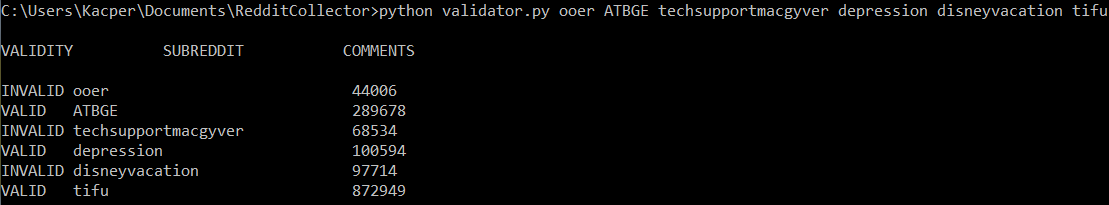
\includegraphics[width=\textwidth]{validator.png}
    \caption{the Subreddit validator in action}
    \label{fig:mesh1}
\end{figure}
Two Subreddits on the list that have not met 100,000 comments have been added to the list regardless, \textit{/r/disneyvacation} at 97,714 comments and \textit{/r/outside} at 95,103 comments.

\section{Statistics}
\section{Similarities between Subreddits}
\section{Conclusions}


\end{document}
